\section{What We Discovered}

\begin{figure}
  \centering
  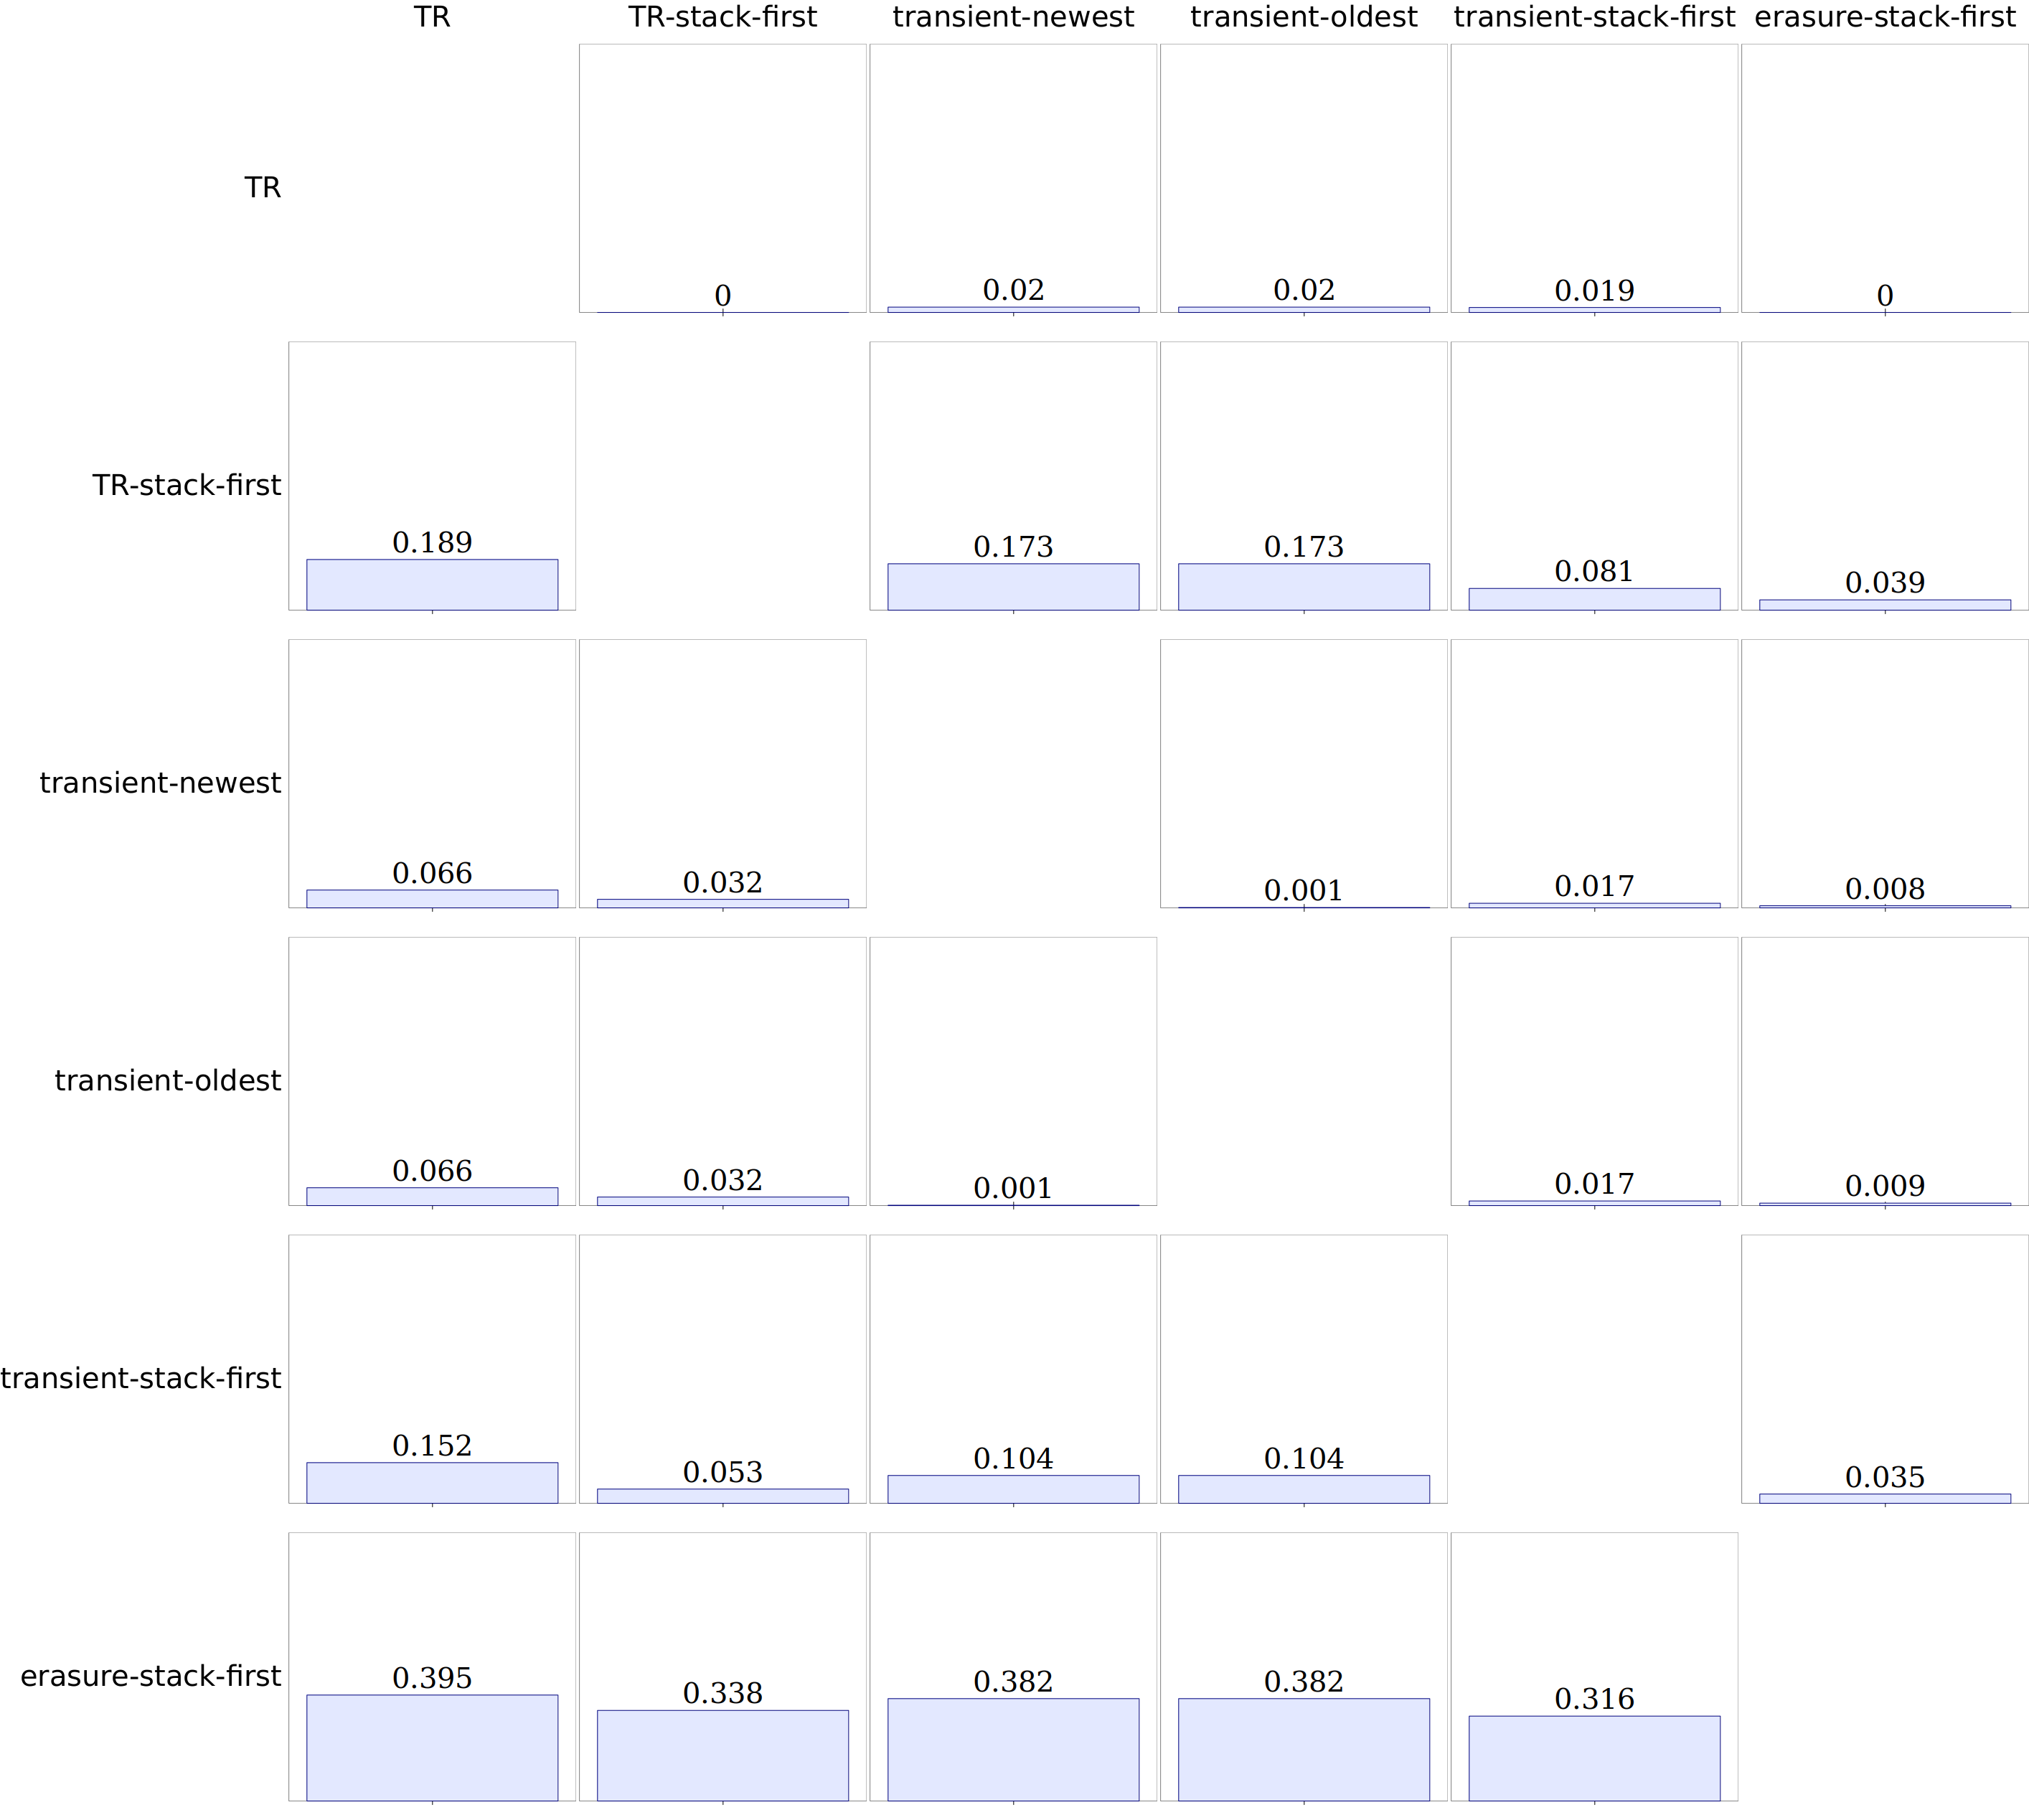
\includegraphics[width=0.45\textwidth]{./plots/avo-matrix}
  \caption{Usefulness comparisons: Each cell depicts the estimated percentage of
  interesting debugging scenarios for which the row mode is more useful
  than the column mode.
  The upper bound of error margin is 0.02\%}
  \label{fig:avo-matrix}
\end{figure}


We run the experimental process from section~\ref{sec:rational} on the
sampled debugging scenarios from section~\ref{sec:sample} on a --- specs
of fix. Each debugging scenario had a timeout limit of 4 minutes and an
out of memory limit of 6GB. The complete experiment required
approximately 270 hours of compute hours on our machine. 


Figure~\ref{fig:avo-matrix} summarizes our results and provides answers to
the four questions from section~\ref{subsec:experiment}.  Specifically, it
depicts a head-to-head comparison of the usefulness of each mode against
every other mode.  The cell in row $R$ and column $C$ plots the percentage
of interesting debugging scenarios for which $R$ is more useful $C$ ---
this percentage has been calculated as an estimated proportion from the
corresponding proportion of the debugging scenarios in our sample and the
upper bound.  In effect, reading across a given row $R$ provides an
overview of how $R$ compares to every other mode; the higher the bars, the
more interesting debugging scenarios for which $R$ is strictly more useful
than the other modes.  Reading down a given row $C$ provides an overview
of how every other mode compares to $C$; the higher the bars, the more
interesting debugging scenarios for which $C$ is strictly less useful than
the other modes. For example, the second cell in the row of Natural blame
shows that Natural is more useful than Natural exceptions for 12\% of all
the interesting debugging scenarios we generate from our benchmarks and
mutators. 

Figure~\ref{subsec:experiment} shows that the answers for questions $Q_1$
to $Q_3$ are positive. In all three semantics, blame modes outperform
their corresponding exception mode (by 9.44\% to 12.7\%). The natural
exceptions mode is never more useful than natural blame and  transient
exceptions are more useful than transient first and transient last blame
in 2.19\% and 2.8\% of the scenarios respectively. 


For the answers to $Q_*$, we compare the percentages in antisymmetric
positions in the matrix. Blame for all three semantics is significantly
more useful than Erasure exceptions (by 33\% to 35\%). Natural blame is
more useful than both versions of transient blame by a small percentage;
in 4.05\% of scenarios natural blame is more useful while in 1.67\% of the
scenarios transient blame is more useful. The transient first and
transient last blame are practically indistinguishable. Finally, there is
no clear winner between natural exceptions and transient exceptions
despite the theoretically advantageous additional checks of the natural
semantics. 

\begin{figure}
  \centering
  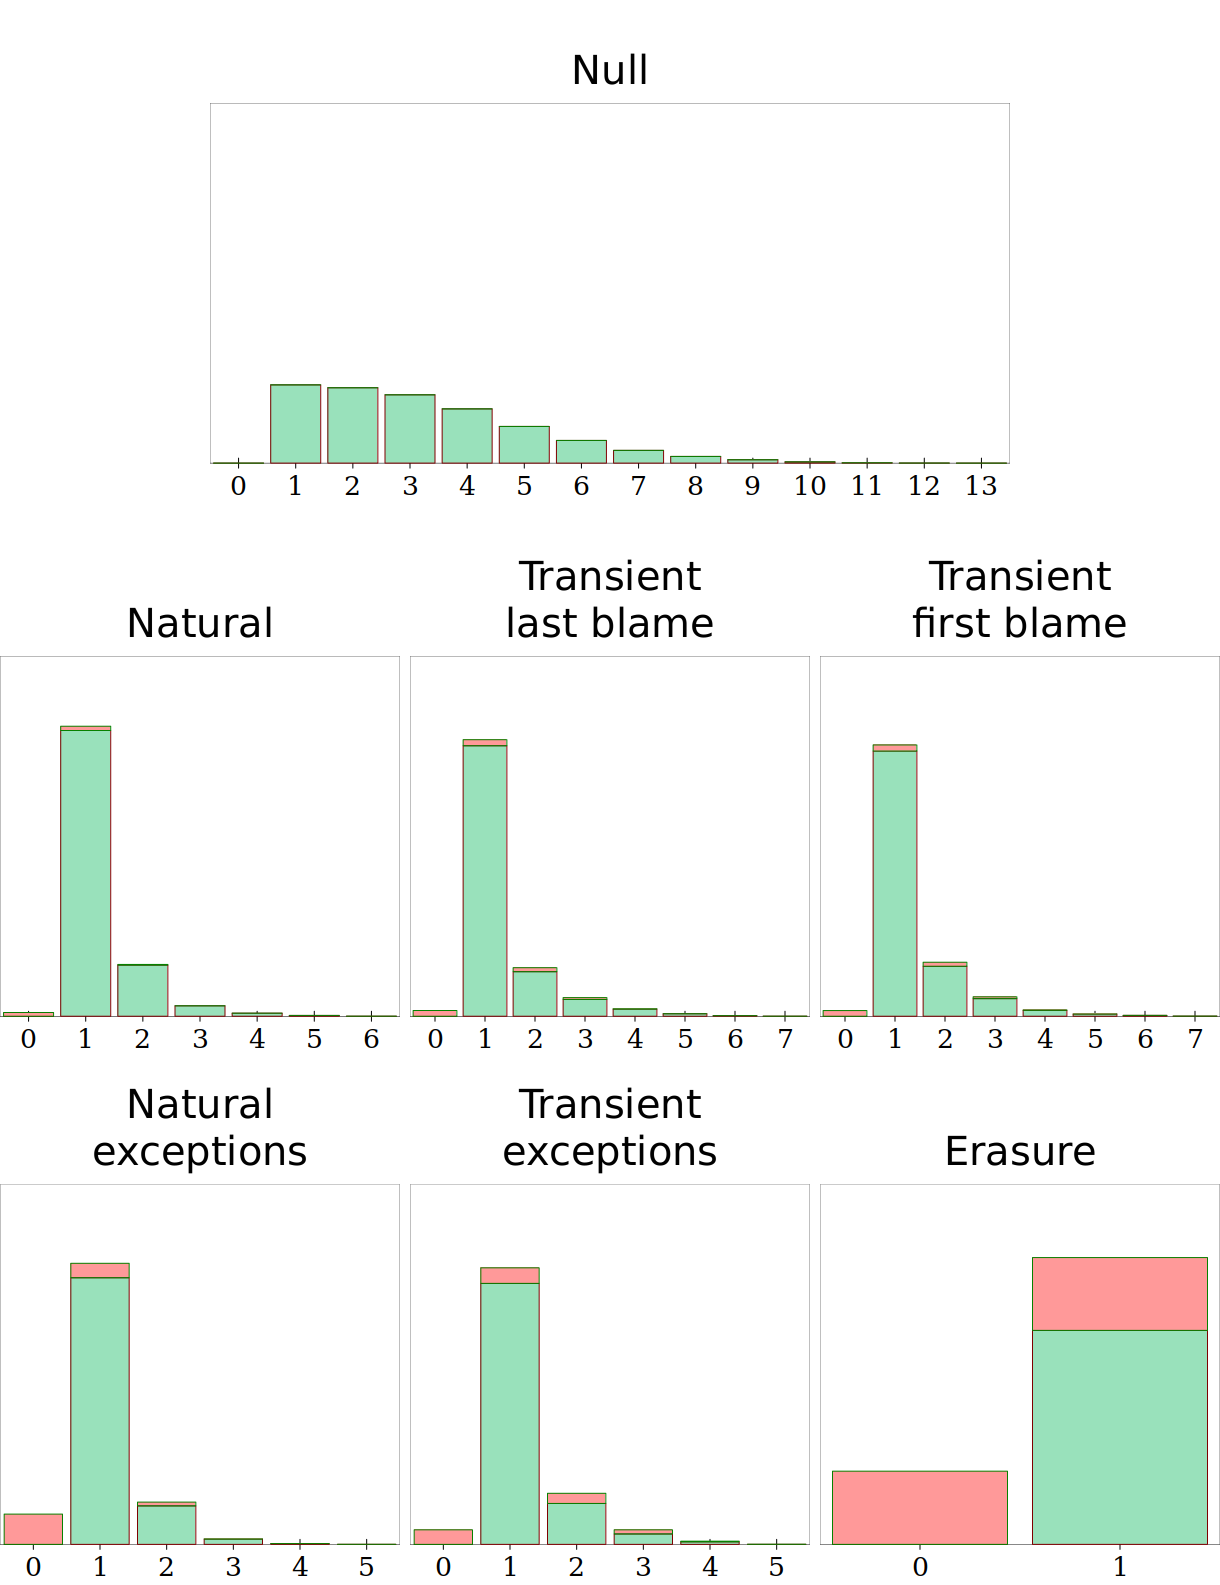
\includegraphics[width=0.4\textwidth]{./plots/bt-lengths-table}
  \caption{Programmer effort: Each plot depicts the distribution of trail
  lengths for a given mode across all benchmarks, starting from trails
  of length 0.}
  \label{fig:effort-table}
\end{figure}


Figure~\ref{fig:effort-table} shows the distribution of programmer effort
for the sampled interesting debugging --- in contrast to the usefulness
comparisons these results do not generalize to the full population. 

